\chapter{Эксперимент СТРЕЛА}
Результаты, приведённые в предыдущей главе были получены на основе
экспериментальных данных со 100-см водородной пузырьковой камеры. Данная камера,
работавшая в пучках лёгких ядер на синхрофазотроне ЛВЭ ОИЯИ, являлась
одновременно чистой протонной мишенью, и детектором вторичных частиц. С её
помощью было проведено большое число исследований, результаты которых
сформулированы в научных статьях. Часть их легла в основу данной диссертации.

Однако, наряду со многими преимуществами, у камерной методики имелся ряд
недостатков, которые накладывали существенные ограничения на затраты труда и
времени для получения физических результатов на современном уровне.

Пузырьковая камера довольно медленный прибор из-за инерционности механических
процессов, изменяющих давление, необходимых для получения чувствительности
перегретой жидкости. Кроме того, накладывают свои ограничения времена,
необходимые для восстановления давления в жидкости и для срабатывания
регистрирующей аппаратуры. Поэтому неуправляемость прибора не позволяет
организовать электронный триггер для отбора интересующих экспериментатора
событий. В одном цикле ускорения нельзя было получить более одной--двух
стереофотографий рабочего объёма камеры.

Другим явным недостатком камерной методики является большая трудоёмкость
обработки полученных снимков. Процесс обработки стереофотографий с пузырьковой
камеры был очень длительным, из-за чего результаты исследований были иногда
статистически мало обеспечены. Несмотря на введение автоматизации при
обработке снимков, статистика изучаемых процессов существенно отставала от
современных электронных экспериментов. В итоге, для получения статистически
обеспеченных результатов, требовались годы (иногда и десятилетия) упорного труда
коллективов.

\section{Предложение электронного эксперимента}
Изучение реакции перезарядки, проведённое с помощью камерной методики, позволило
предложить схему электронного эксперимента. По мере развития электронных методов
регистрации частиц (и наличия пучка дейтронов) появилась возможность изучения
интересующего нас процесса при использовании выведенного пучка ускоренных
дейтронов на Нуклотроне ЛФВЭ ОИЯИ. В работе~\cite{glagolev96} было впервые
предложено исследование зарядово-обменных процессов в дейтрон-протонных
соударениях на ускорителе Нуклотрон с целью изучения спиновых эффектов в
неполяризованных пучках дейтронов с помощью электронной методики, для получения
статистически обеспеченного результата по определению вклада спин-зависящей
части амплитуды элементарного $np$-рассеяния.

В предлагаемом эксперименте требуется наблюдать события dp-взаимодействий с
вылетом из мишени двух протонов с близкими импульсами в переднем направлении,
т.е. при малых переданных импульсах. В области энергий 1~ГэВ и выше, на момент
формулирования предложения, практически отсутствовали экспериментальные данные
отношения $R_{\np}$ дифференциальных сечений для реакции перезарядки на дейтроне
и реакции элементарной перезарядки нейтрона на протоне.

Нами была предложена~\cite{bush00_mucha,glagolev00_mucha} довольно простая схема
эксперимента (изучается процесс с малой множественностью вторичных частиц и
предсказуемой кинематикой), а именно~--- использование одноплечевого
спектрометра с достаточно узкой апертурой, изображённая на
рис.~\ref{fig:strela_scheme}. Пучок дейтронов падает на мишень, анализирующий
магнит разводит в пространстве вторичные заряженные частицы протоны (или
$\pi$-мезоны) и непровзаимодействовавшие дейтроны. Основным конкурирующим
процессом при выделении реакции перезарядки (двухпротонные события) является
реакция прямого развала дейтрона (однопротонные события), которая в свою очередь
служит дополнительным калибровочным процессом~\cite{are_mucha04}.

\begin{figure}[h]
  \centering
  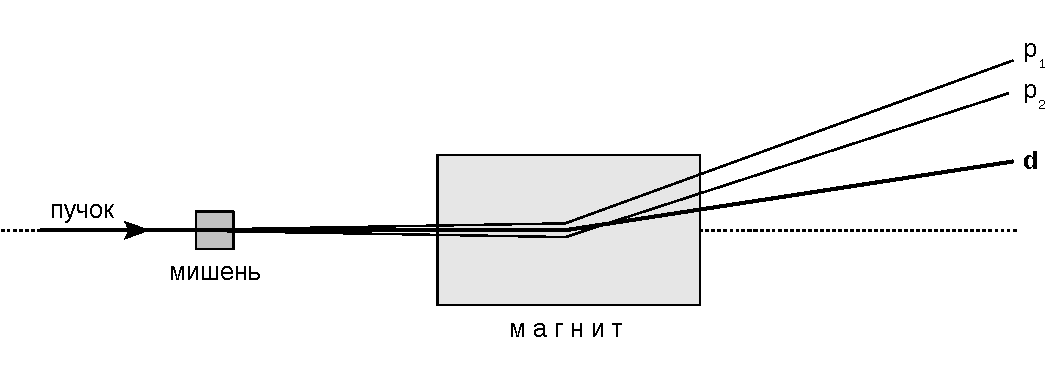
\includegraphics[width=1.00\textwidth]{strela_scheme.pdf}
  \caption{Схема эксперимента с использованием одноплечевого спектрометра,
    обеспечивающая отбор событий с вылетом из мишени двух протонов с близкими
    импульсами в переднем направлении.}
  \label{fig:strela_scheme}
\end{figure}

Предлагаемая \! схема электронного эксперимента позволяет регистрировать пары
протонов с малым углом раствора, имеющие импульс равный приблизительно половине
импульса дейтрона. Этим обеспечивается отбор событий под нулевым углом по
отношению к первичному пучку, что соответствует небольшому переданному импульсу
рассеянному протону ($t \simeq 0$) и малым относительным импульсам внутреннего
движения нуклонов в дейтроне. Таким образом, реализуются необходимые условия для
выделения предполагаемого процесса.

Выбор конкретной геометрии эксперимента был выполнен на основе реальных событий
и расчётов методом генерации Монте"--~Карло с помощью программного пакета GEANT.
Опираясь на данные по реакции $dp \rightarrow X$, полученные на водородной
пузырьковой камере, был промоделирован вариант эксперимента для спектрометра,
используя в качестве входных данных реальные события $dp$-взаимодействий. Для
оценки фоновых условий были взяты все 17 наблюдавшихся каналов реакций
(таблица~\ref{tab:dp_channels}) информация о которых содержится на DST камерного
эксперимента. Фон от других реакций, кроме изучаемой реакции \dpfrag, которые
могли дать два положительно заряженных трека (например
$dp \rightarrow ppn\pi^{0}$) в направлении вперёд при ограниченной апертуре
оказался пренебрежимо малым~\cite{baz99}.

В результате была предложена схема экспериментальной установки
СТРЕЛА~\cite{strela_web}. Были необходимы детекторы с хорошим пространственным
разрешением и быстрая современная электроника для считывания большого потока
информации. В качестве трековых детекторов были выбраны дрейфовые камеры. Не
менее важной задачей был выбор системы отбора и регистрации событий. Особые
требования предъявляются и к характеристикам выведенного из ускорителя и
транспортируемого на мишень пучка дейтронов. Трудности предлагаемой схемы
заключаются в необходимости получения равномерной временной структуры (временная
растяжка пучка в несколько секунд) и ограниченной интенсивности пучка,
фокусируемого на мишень, для уменьшения доли случайных совпадений и минимизации
сбоев в работе дрейфовых камер. В следующих разделах подробно описывается
созданная экспериментальная установка СТРЕЛА.

\section{Описание установки СТРЕЛА}
Экспериментальная установка СТРЕЛА предназначена для исследования
зарядово-обменных процессов во взаимодействиях дейтронов с протонами в области
энергий выше 1~ГэВ. Установка представляет собой одноплечевой магнитный
спектрометр, который расположен в зале корпуса \No205 ЛФВЭ ОИЯИ,
рис.~\ref{fig:strela_205}. Пучок дейтронов, выведенный из ускорителя Нуклотрон,
транспортируется и фокусируется магнитной оптикой канала ВП-1 на мишень
установки, которая находится в области перед фокусом Ф5~\cite{issinsky94}.
Канал транспортировки выведенного пучка состоит из поворотных магнитов и
дублетов магнитных линз, рис.~\ref{fig:channel_VP1}.

\begin{figure}[h]
  \centering
  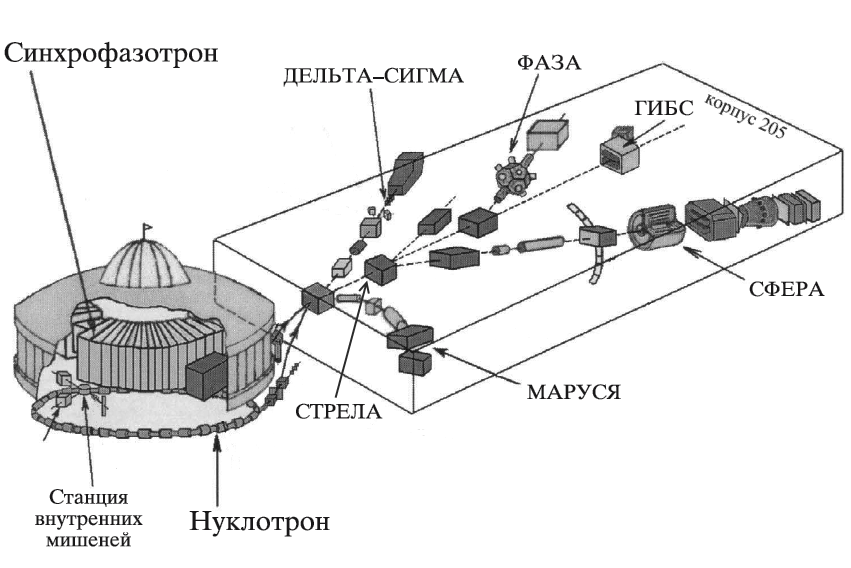
\includegraphics[width=1.00\textwidth]{strela_205.png}
  \caption{Схема ускорительного комплекса ЛФВЭ ОИЯИ Нуклотрон с базовыми
    установками. Установка СТРЕЛА расположена в зале корпуса \No205.}
  \label{fig:strela_205}
\end{figure}

\begin{figure}[h]
  \centering
  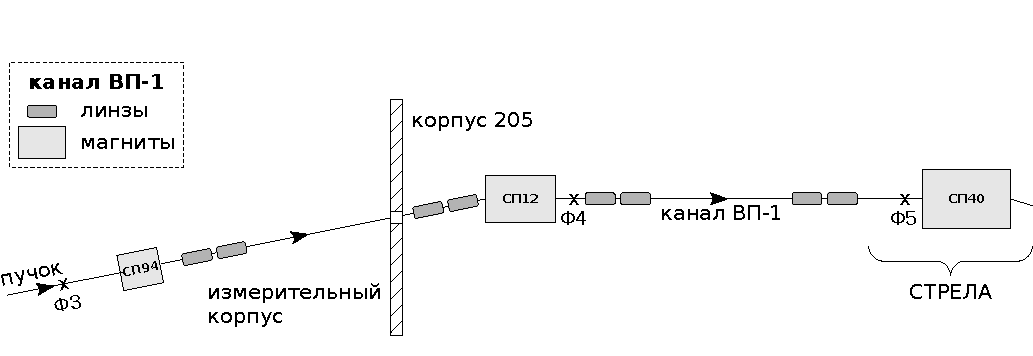
\includegraphics[width=1.00\textwidth]{channel_VP1.pdf}
  \caption{Канал ВП-1 выведенного пучка из ускорителя Нуклотрон с фокусами
    Ф3--Ф5. Транспортировка дейтронного пучка, до мишени установки СТРЕЛА,
    обеспечивается отклоняющими дипольными магнитами и фокусирующими
    квадрупольными линзами.}
  \label{fig:channel_VP1}
\end{figure}

\noindent
Основными элементами установки СТРЕЛА являются:
\begin{itemize}
\item блоки дрейфовых камер в качестве координатных детекторов,
\item электроника считывания информации,
\item сцинтилляционные счётчики используемые для запуска установки,
\item анализирующий магнит.
\end{itemize}

Для определения координат траекторий первичной и вторичных частиц в эксперименте
применяются дрейфовые камеры, которые объединяются в блоки. На
рис.~\ref{fig:strela_setup} приведена схема расположения всех блоков дрейфовых
камер, анализирующего магнита, мишени и сцинтилляционных (триггерных) счётчиков
на выведенном пучке дейтронов из ускорительного комплекса Нуклотрона.

\begin{figure}[h]
  \centering
  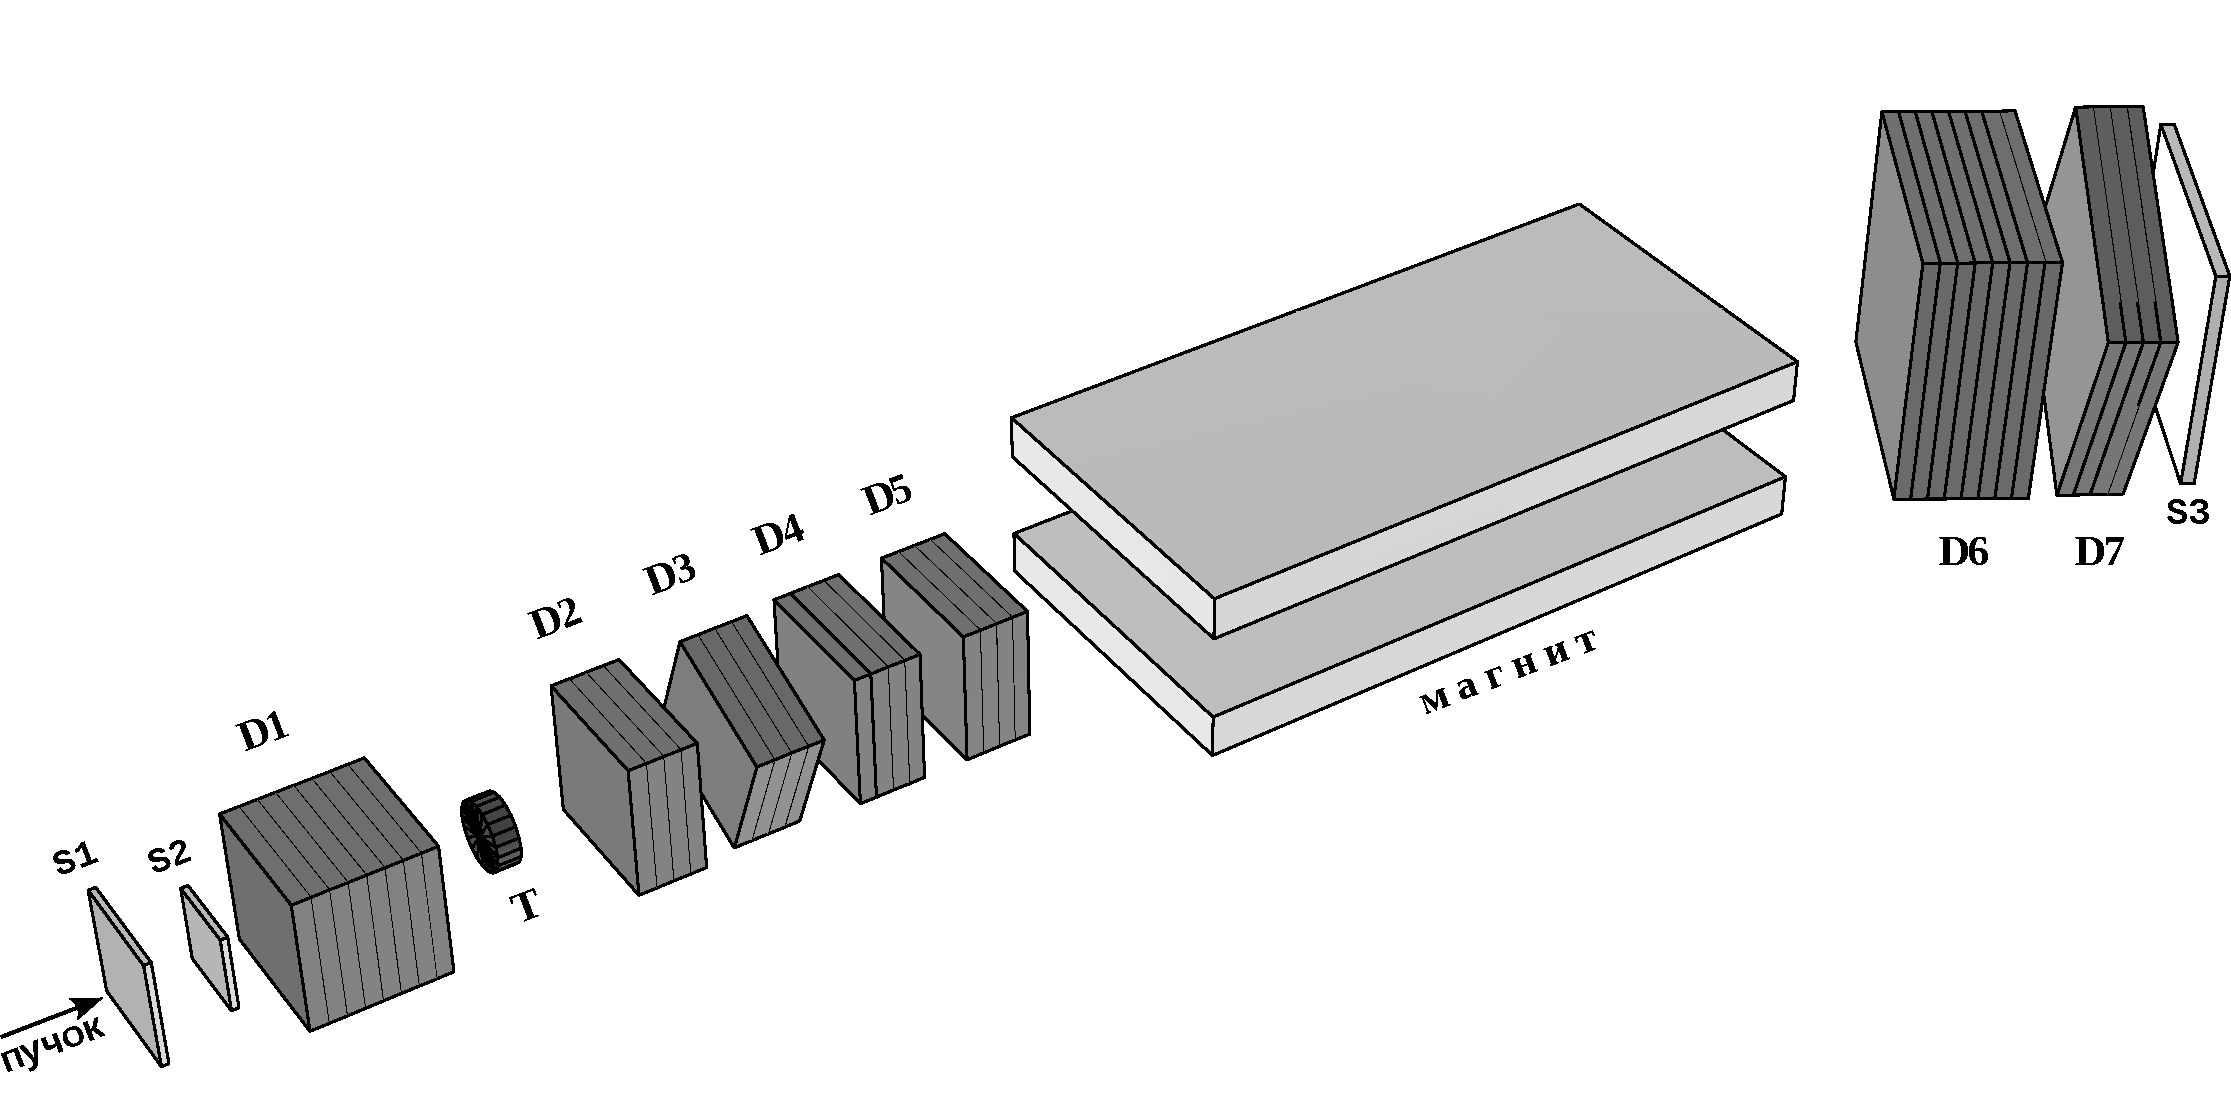
\includegraphics[width=1.00\textwidth]{strela_setup.pdf}
  \caption{Схема расположения дрейфовых камер и анализирующего магнита на
    экспериментальной установке СТРЕЛА. D1--D5~--- блоки <<маленьких>> дрейфовых
    камер с размером рабочей области 12.5~$\times$~12.5~см$^2$, D6--D7~---
    блоки <<больших>> камер с размером 25.0~$\times$~25.0~см$^2$, S1--S3~---
    сцинтилляционные счётчики,  Т~--- мишень.}
  \label{fig:strela_setup}
\end{figure}

В настоящее время используется 36 плоскостей дрейфовых камер, объединённых в 7
блоков. Каждый блок состоит из четырёх или восьми объединённых плоскостей
дрейфовых камер с различной ориентацией проволочек.

Длина дрейфового промежутка во всех камерах равна 21~мм.  Камеры в блоке
располагаются таким образом, что сигнальные проволочки в соседних плоскостях
сдвинуты относительно друг друга на 21~мм в направлении перпендикулярном оси
пучка. Такое расположение нитей позволяет устранить лево-правую неоднозначность
в определении пространственных координат треков частиц.

Координатная система дрейфовых камер выбрана следующим образом: ось $z$ для
блоков камер D1--D5 направлена по пучку падающих дейтронов, а для блоков камер
D6--D7, помещённых после магнита, по направлению максимума вылета протонов
стриппинга; оси $x$ и $y$ лежат в плоскостях камер так, что вместе с осью $z$
составляют правую тройку; координаты $u$ и $v$ используются для повёрнутых камер
вместо $x$ и $y$.

В таблице~\ref{tab:cham_config} приведена структура всех блоков дрейфовых камер
с их регистрируемыми координатами и количеством сигнальных проволочек в каждой
плоскости камеры, штриховая координата используется для сдвинутых проволочек.
\newcolumntype{M}{>{\columncolor[gray]{0.75}[0.90\tabcolsep]}c}
\begin{table}[h]
  \begin{center}
    \bigskip
    \resizebox{1.0\textwidth}{!} {
      \begin{tabular}{|l|c|c|c|c|c|c|c|c|c|c|c|c|c|c|c|c|}
        \hline
        Расположение блока & \multicolumn{16}{c|}{До мишени} \\
        \hline
        Блок & \multicolumn{4}{c|}{} &
        \multicolumn{8}{M|}{D1} & \multicolumn{4}{c|}{} \\
        \cline{6-13}
        Координата & \multicolumn{4}{c|}{} &
        $y$ & $y\,'$ & $y$ & $y\,'$ & $x$ & $x\,'$ & $x$ & $x\,'$ &
        \multicolumn{4}{c|}{} \\
        Число проволочек & \multicolumn{4}{c|}{} &
        4 & 3 & 4 & 3 & 4 & 3 & 4 & 3 & \multicolumn{4}{c|}{} \\
        \hline \hline

        Расположение блока & \multicolumn{16}{c|}{За мишенью} \\
        \hline
        Блок & \multicolumn{4}{M|}{D2} & \multicolumn{4}{M|}{D3} &
        \multicolumn{4}{M|}{D4} & \multicolumn{4}{M|}{D5} \\
        \cline{2-17}
        Координата & $y$ & $y\,'$ & $x$ & $x\,'$ & $u$ & $u\,'$ & $v$ & $v\,'$ &
        $x$ & $x$ & $x\,'$ & $x\,'$ & $y$ & $y\,'$ & $x$ & $x\,'$ \\
        Число проволочек &
        4 & 3 & 4 & 3 & 4 & 3 & 4 & 3 & 4 & 4 & 3 & 3 & 4 & 3 & 4 & 3 \\
        \hline \hline

        Расположение блока & \multicolumn{16}{c|}{За магнитом} \\
        \hline
        Блок & \multicolumn{2}{c|}{} & \multicolumn{8}{M|}{D6} &
        \multicolumn{4}{M|}{D7} & \multicolumn{2}{c|}{} \\
        \cline{4-15}
        Координата & \multicolumn{2}{c|}{} &
        $y$ & $y\,'$ & $y$ & $y\,'$ & $x$ & $x\,'$ & $x$ & $x\,'$ & $u$ & $u\,'$
        & $v$ & $v\,'$ &
        \multicolumn{2}{c|}{} \\
        Число проволочек & \multicolumn{2}{c|}{} &
        7 & 6 & 7 & 6 & 7 & 6 & 7 & 6 & 7 & 6 & 7 & 6 & \multicolumn{2}{c|}{} \\
        \hline
      \end{tabular}
    }
    \smallskip
    \caption{Конфигурация блоков дрейфовых камер на установке
      СТРЕЛА. $uv$-координаты повёрнутые относительно $xy$-координат вокруг оси
      $z$, штриховая координата означает сдвинутую плоскость камеры.}
    \label{tab:cham_config}
  \end{center}
\end{table}



%%% Local Variables:
%%% mode: latex
%%% TeX-master: "../musinsky_disser"
%%% coding: utf-8
%%% End:


До мишени располагается первый блок дрейфовых камер (D1) с размером рабочей
области 12.5~$\times$~12.5~см$^2$, имеющий четыре плоскости $y$-координат и
четыре плоскости $x$-координат. Первый блок служит для определения треков
пучковых дейтронов, падающих на мишень.

За мишенью располагаются четыре блока дрейфовых камер с такими же размерами
(<<маленькие>> камеры). Первый блок (D2) имеет две плоскости $y$-координат и две
плоскости $x$-координат, второй блок (D3)~--- две плоскости $u$-координат и две
плоскости $v$-координат. $uv$-координаты повёрнуты на 22.5$^{\,\circ}$
относительно $xy$-координат вокруг оси $z$, проходящей через центры блоков камер
в направлении падающего пучка. Далее следует блок дрейфовых камер (D4) с
четырьмя плоскостями $x$-координат, и последний блок (D5) имеет две плоскости
$y$-координат и две плоскости $x$-координат. Такой набор камер после мишени
позволяет надёжно идентифицировать два близко проходящих трека. Расстояние между
центрами двух крайних блоков D2 и D5 равно 65~см, между блоком D1 и блоком D2,
расположенными до и за мишенью, равно 90~см.

За анализирующим магнитом располагаются два блока дрейфовых камер с размерами
рабочей области 25.0~$\times$~25.0~см$^2$ (<<большие>> камеры). Ось $z$ данных
блоков (D6--D7) повёрнута на угол приблизительно~14$^{\,\circ}$ относительно оси
$z$ блоков камер (D1--D5), которые расположены перед отклоняющим магнитом.
Первый блок (D6) имеет четыре плоскости $y$-координат и четыре плоскости
$x$-координат, а второй блок (D7)~--- две плоскости $u$-координат и две
плоскости $v$-координат (повёрнутых также на 22.5$^{\,\circ}$ относительно
$xy$-координат). Расстояние между центрами блоков дрейфовых камер D6 и D7 равно
30~см.

Число всех регистрируемых сигналов с проволочек составляет 162. На каждой камере
установлены платы с микросхемами, в которых осуществляется усиление,
формирование и дискриминация входных сигналов от сигнальных проволочек дрейфовых
камер. Сформированные сигналы поступают на входы TDC модулей для оцифровки.
Полученная информация передаётся по оптической линии в персональный компьютер
для дальнейшей обработки.

Дрейфовые камеры являются основным элементом \! экспериментальной установки
СТРЕЛА. Перейдём теперь к более детальному описанию принципов их работы,
конструкции, характеристикам и электронной системе считывания информации с
сигнальных проволочек.

\section{Дрейфовые камеры}
Дрейфовые камеры применяются в физических экспериментах уже почти сорок
лет. Шарпак и его группа впервые предложили идею использовать измерение времени
дрейфа для определения координаты частиц в конце 60-х годов прошлого
века~\cite{charpak68,charpak93}. Дрейфовые камеры стали одним из базовых видов
координатных детекторов на многих установках по физике высоких энергий во всём
мире. Основным преимуществом является высокое пространственное разрешение и
относительно несложная конструкция.

Дрейфовая камера~--- это газонаполненный координатный детектор заряженных
частиц. Координата регистрируемой частицы определяется по времени дрейфа
электронов в газе. Внутри камеры натянуто большое число проволочек, которые
находятся под напряжением. Расположение проволочек выбрано таким образом, чтобы
в пространстве между ними возникало однородное электрическое поле.

Заряженная частица, пролетающая через рабочий объём камеры, оставляет
ионизационный след. Электроны под действием сил электрического поля в камере
движутся с почти постоянной скоростью (дрейфуют) вдоль направления поля к
сигнальным проволочкам, и по достижении ими проволочки, электроника камеры
передаёт на выход сигнальный импульс. По сигналам с проволочек можно с
достаточно хорошей точностью восстановить координаты пролетевшей заряженной
частицы.

\subsection{Ионизация и дрейф электронов в газах}
Основные потери энергии быстрых заряженных частиц происходят в результате
кулоновского взаимодействия при столкновениях с атомными электронами. Заряженная
частица или возбуждает атом, или ионизирует, при этом теряет энергию.
Ионизационные потери энергии на единицу длины пути определяются формулой
Бете"--~Блоха~\cite{pdg08}.

Ионизационное торможение~--- главный механизм потерь энергии при прохождении
быстрой заряженной частицы через вещество детектора. В газовых детекторах, таких
как дрейфовые камеры, вклад от других процессов (тормозное, переходное или
черенковское излучения) в полную потерю энергии частицы незначителен.

Заряженная частица, проходящая через рабочий объём камеры, в результате
ионизации образует электроны и положительные ионы. Они быстро теряют свою
энергию при многократных столкновениях с окружающими атомами и молекулами
рабочего газа, распределение по энергии близко тепловому.

Со временем плотность образованного заряда уменьшается из-за рекомбинации
(нейтрализации положительных и отрицательных ионов) и электронного захвата
(возможности захватывать электроны низких энергий некоторыми многоатомными
молекулами). Вероятность такого захвата характеризуется коэффициентом
прилипания, который для электроотрицательных газов, таких как $O_2$, $CO_2$ и
$Cl_2$, достаточно велик, но пренебрежимо мал для таких газов как $N_2$, $H_2$,
$Ar$ или $CH_4$~\cite{klajk90}.

Если образовавшиеся ионы подвергаются воздействию электрического поля с
напряжённостью $E$, они начинают двигаться вдоль линий электрического
поля. Электроны по направлению поля к анодным проволочкам, а положительные ионы
к катодам. Средняя скорость движения электронов и ионов называется скоростью
дрейфа, её можно записать в виде $v_d = \mu E$, где $\mu$~--- подвижность
ионов, которая кроме напряжённости $E$ в~электрическом поле, зависит также от
состава газовой смеси, давления и температуры. На рис.~\ref{fig:drift_velocity}
показаны зависимости скорости дрейфа электронов от напряжённости электрического
поля для различных газов при нормальных условиях~\cite{sauli02}. Видно, что
скорость дрейфа для разных газов может отличаться на порядок. Кроме того
желательно использовать газ, в котором при достаточной напряжённости
электрического поля, скорость дрейфа слабо меняется при изменении поля.

\vspace{-0.5cm}
\begin{figure}[h]
  \centering
  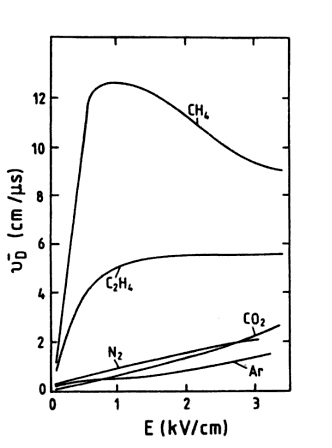
\includegraphics[width=0.55\textwidth]{drift_velocity.png}
  \caption{Зависимость скорости дрейфа электронов $v_d$ от напряжённости
    электрического поля $E$ в некоторых смесях газа при нормальных условиях.}
  \label{fig:drift_velocity}
\end{figure}

Подвижность электронов в газах на несколько порядков больше подвижности ионов
при той же самой напряжённости электрического поля~\cite{pesehonov86}.
Электроны, при достаточно большом значении $E$, смогут за время между двумя
столкновениями, приобрести в электрическом поле энергию, достаточную для
вторичной ионизации атомов газа, произойдёт газовое усиление. В результате число
носителей зарядов возрастает. При высоких значениях $E/p$, где $p$~--- давление
в газе, число новых электронов растёт лавинообразно.

Количество вторичных электронов $\alpha$, образованных в лавине одним электроном
на пути длины 1 см вдоль линии электрического поля, называется первым
коэффициентом Таунсенда, или коэффициентом ударной ионизации. Если $N_0$~---
число первичных электронов, созданных ионизирующей частицей, то полное число
электронов $N(x)$ в точке лавины $x$ равно $N(x) = N_0\,e^{\,\alpha\,x}$.
Коэффициент газового усиления $u$ можно определить как
\begin{equation}
  u\,=\,\frac{N}{N_0}\,=\,e^{\,\int \alpha(x)\,dx}\,.
\end{equation}
На рис.~\ref{fig:gas_townsend} показана зависимость коэффициента Таунсенда от
значения отношения $E/p$. Видно, что развитие лавины в газах, обычно
используемых в дрейфовых камерах, начинается при значении $E/p$ приблизительно
100~В/см~торр~\cite{rope04}.

\begin{figure}[h]
  \centering
  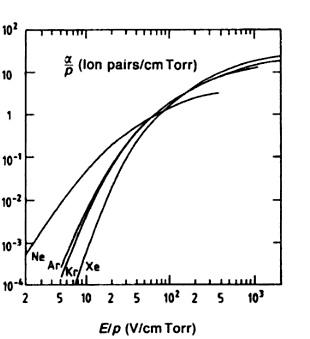
\includegraphics[width=0.55\textwidth]{gas_townsend.png}
  \caption{Зависимость первого коэффициента Таунсенда от значения $E/p$ для
    разных инертных газов.}
  \label{fig:gas_townsend}
\end{figure}

Рабочие газы, используемые в камерах, должны иметь высокий коэффициент газового
усиления. При использовании инертных (благородных) газов, можно получить эффект
газового усиления и при более низкой напряжённости электрического поля. В таких
газах электрон в основном теряет энергию на ионизацию, а не на возбуждение.
В большинстве случаев применяется аргон или ксенон с различными добавками, в
качестве которых чаще всего используется изобутан, метан или
углекислота~\cite{zanevski78}.

Ионизирующая частица, проходящая через дрейфовую камеру, образует вдоль своего
пути свободные электроны, которые зарождают лавины. Заряд рождается в
непосредственной близости от анодной проволочки в области сильного
электрического поля. Сигнал с каждой проволочки регистрируется отдельно, что
позволяет определить координату частицы в камере.

\subsection{Плоская дрейфовая камера}
Идея определения координаты регистрируемой частицы, вызывающей ионизацию газа,
измерением времени дрейфа первичных электронов в однородном электрическом поле,
была высказана уже вскоре после появления многопроволочной пропорциональной
камеры~\cite{charp70}.

Разница во времени $\delta t$ определяется между моментом первичной ионизации
(прохождением частицы) $t_0$ и моментом, когда электроны достигают анодной
проволочки (попаданием облака заряда) $t_1$. Координату $x$ места прохождения
частицы в направлении нормальном к плоскости анодных проволочек в дрейфовой
камере, можно потом вычислить с помощью следующего выражения как
\begin{equation}
  x=\int_{t_0}^{t_1} v_d\,\delta t\,,
\end{equation}
где $v_{d}$~--- скорость дрейфа электронов в газе, которая не должна меняться,
но должна быть достаточно высокой для повышения быстродействия
камеры~\cite{sauli77}.

Для точного измерения координат трековой частицы, необходимо достичь постоянной
скорости дрейфа электронов и линейной зависимости времени дрейфа от координаты
прохождения частицы по всему объёму камеры. Желательную постоянную скорость
дрейфа  можно реализовать созданием постоянной напряжённости электрического поля
вдоль пути дрейфующего электрона. Между соседними сигнальными проволочками
находящимися под потенциалом $+\,U_1$ вводятся дополнительные потенциальные
проволочки под потенциалом $-\,U_2$. На катодные проволочки подан равномерно
распределённый потенциал от 0 до~$-\,U_2$. Данное условие достигается с высокой
точностью практически по всему рабочему объёму дрейфовой камеры, кроме областей
близких к сигнальным проволочкам и на краю камеры, из-за сильного градиента
электрического поля.

Стабильность скорости дрейфа обеспечивается также правильным подбором газовой
смеси. В ряде газовых смесей удаётся обеспечить требуемую скорость дрейфа в
широком диапазоне напряжений~\cite{peisert84}.Тем не менее на изменение
дрейфовой скорости электронов оказывает влияние ряд внешних факторов, таких как
температура, влажность, атмосферное давление или внешнее магнитное поле. Однако
при соблюдении определённых условий можно достичь стабильной работы камер
(постоянную скорость дрейфа электронов) в течение длительного времени
эксперимента.

Пространственное разрешение дрейфовых камер можно выразить как погрешность в
измерении координаты траектории частицы, которая определяется однородностью
электрического поля в области дрейфа. Ограничение на итоговое разрешение вносит
ещё ряд факторов: временное разрешение электроники, неточности при изготовлении
камеры, диффузия электронов во время их дрейфа к аноду, статистическая
флуктуация первичной ионизации в близости анодной проволочки,
рис.~\ref{fig:resolution_cham}~\cite{sitar87}. Кроме того, пространственное
разрешение ухудшается, в зависимости от угла наклона проходящей частицы к
плоскости камеры. Для очень больших наклонов треков оно может упасть почти в
два раза.

\begin{figure}[h]
  \centering
  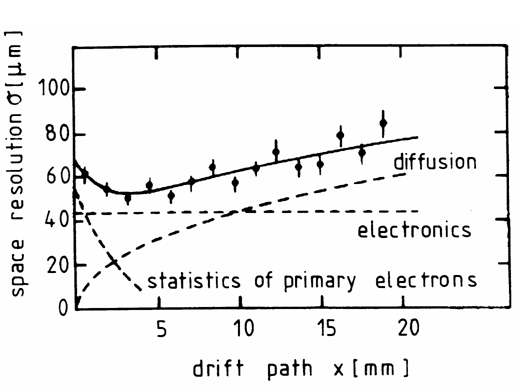
\includegraphics[width=0.80\textwidth]{resolution_cham.png}
  \caption{Пространственное разрешение дрейфовой камеры $\sigma$ в зависимости
    от длины дрейфа электронов $x$.}
  \label{fig:resolution_cham}
\end{figure}

\section{Конструкция дрейфовой камеры}
На экспериментальной установке СТРЕЛА используются два вида дрейфовых камер.
Камеры с размером рабочей области 12.5~$\times$~12.5~см$^2$ (маленькие камеры),
внутри которых натянуты три или четыре сигнальные проволочки, и камеры с
размером 25.0~$\times$~25.0~см$^2$ (большие камеры), имеющие шесть или семь
сигнальных проволочек. Конструкции камер обоих размеров аналогичны.

Одна дрейфовая камера имеет три плоскости проволочных электродов: плоскость
сигнальных и потенциальных проволочек и две плоскости катодов. Принципиальная
схема расположения проволочек дрейфовой камеры показана на
рис.~\ref{fig:cham_wires}.

\begin{figure}[h]
  \centering
  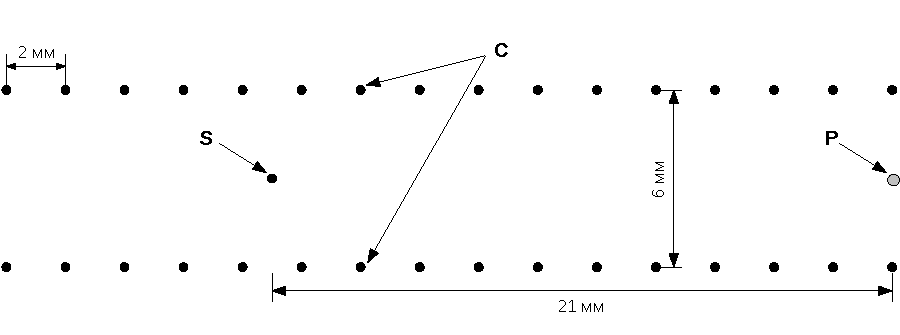
\includegraphics[width=0.95\textwidth]{cham_wires.pdf}
  \caption{Конфигурация проволочек дрейфовой камеры. S~--- сигнальная
    проволочка, P~--- потенциальная проволочка, C~--- катодные проволочки.
    Расстояние между сигнальной и потенциальной проволочками равно 21~мм,
    расстояние между двумя плоскостями катодов 6~мм и шаг намотки между
    катодными проволочками 2~мм.}
  \label{fig:cham_wires}
\end{figure}

Расстояние между двумя соседними сигнальными проволочками равно 42~мм, что
соответствует максимальному дрейфовому промежутку 21~мм. Расстояние между
катодными плоскостями равно 6~мм, шаг намотки катодных электродов 2~мм.
Потенциальные и сигнальные нити, расстояние между которыми 21~мм, расположены в
плоскости, равноотстоящей от катодов~\cite{vodopianov84}.

Для полеобразующих катодных электродов использовалась нить из бериллиевой бронзы
диаметром 100~мкм. Намотка катодных плоскостей проводилась на намоточном станке,
что позволило обеспечить высокую точность укладки проволочек $\pm 15$~мкм.
Сигнальные и потенциальные проволочки, припаянные к соответствующим проводникам
сигнальных и потенциальных печатных электродов, ставились в заданные позиции с
точностью $\pm 10$~мкм под микроскопом. Сигнальные нити~--- золочённая
вольфрамовая проволока диаметром 20~мкм. Потенциальные нити~--- посеребрённая
проволока из бериллиевой бронзы диаметром 60~мкм. Натяжение проволок на уровне
50~грамм~\cite{nigmanov76}.

Расстояние между плоскостью катодных электродов и плоскостью сигнальных и
потенциальных проволочек равно 3~мм. Эквидистантное междуэлектродное
расстояние обеспечивается калибровочными планками, которые приклеены к плоскости
катодных проволочных электродов.

\begin{figure}[h]
  \centering
  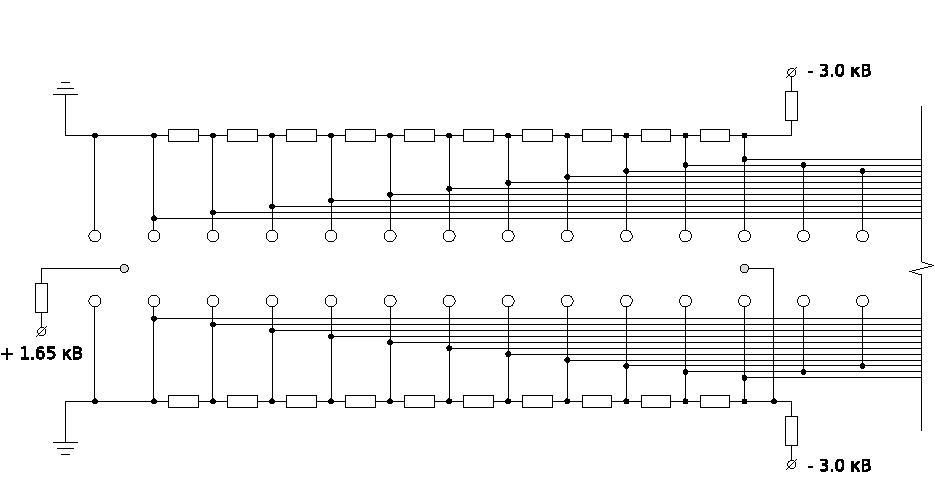
\includegraphics[width=1.0\textwidth]{cham_voltage.pdf}
  \caption{Схема распределения электрического напряжения в дрейфовой камере.
    На сигнальную проволочку подаётся положительный потенциал $+1.65$~кВ, на
    потенциальную $-3.0$~кВ. На катодные проволочки подан равномерно
    распределённый потенциал от $-3.0$~кВ до 0.}
  \label{fig:cham_voltage}
\end{figure}

Распределение напряжённости электрического поля в дрейфовой камере формируется
проволочными электродами. \! Потенциал катодов распределён с помощью резистивных
делителей равномерно от максимального $-3.0$~кВ до нуля. На сигнальные
проволочки подаётся положительный потенциал $+1.65$~кВ, на потенциальные нити
максимальный катодный потенциал $-3.0$~кВ, рис.~\ref{fig:cham_voltage}. Данная
конструкция (в сочетании с газовой смесью) обеспечивает почти постоянную
напряжённость электрического поля $\sim 1.5$~кВ/см вдоль пути дрейфа электронов,
образованных ионизацией среды пролетающей заряженной частицей.

Лево-правая неоднозначность является недостатком при использовании дрейфовых
камер и не позволяет определить, с какой именно стороны пролетела регистрируемая
частица относительно сигнальной проволочки. Неоднозначность устраняется сдвигом
(смещением) соседних плоскостей камер так, чтобы сигнальные проволочки были
сдвинуты относительно друг друга на 21~мм, т.е. на половину расстояния между
ними в направлении перпендикулярном оси пучка. Прямой дрейфовой камерой,
называем камеру имеющую четыре сигнальных и три потенциальных проволочки (для
большой камеры семь сигнальных и шесть потенциальных), сдвинутая камера имеет
три сигнальных и четыре потенциальных проволочки (большая камера шесть
сигнальных и семь потенциальных).

\subsection{Блок дрейфовой камеры}
Блок дрейфовой камеры объединяет несколько плоскостей (слоёв) дрейфовых камер с
различной ориентацией сигнальных проволочек. На установке применяется семь
блоков дрейфовых камер, каждый из которых имеет четыре или восемь плоскостей.
Структура отдельных блоков с их регистрируемыми координатами и числом сигнальных
проволочек указана в таблице~\ref{tab:cham_config}.

На рис.~\ref{fig:cham_block_construct} приведено схематическое изображение
одного блока дрейфовой камеры (показаны только две плоскости камер). Основные
конструктивные элементы блока камеры:
\begin{itemize}
\item рамка камеры,
\item проволочные электроды,
\item печатные электроды.
\end{itemize}

\begin{figure}[h]
  \centering
  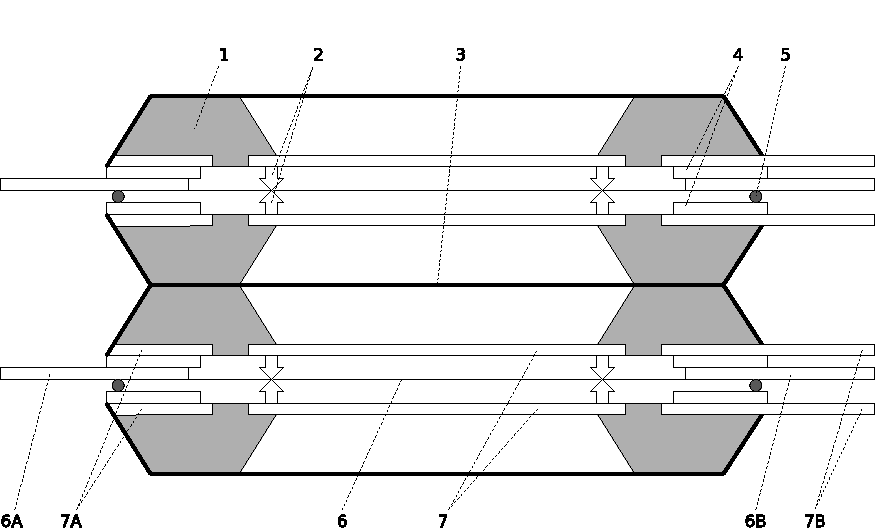
\includegraphics[width=1.00\textwidth]{cham_block_construct.pdf}
  \caption{Изображение одного блока дрейфовой камеры (две плоскости камер).
    1~--- рамка из эпоксидного компаунда, 2~--- калибровочные планки, 3~---
    разделительный проволочный электрод, 4~--- разделительные полосы, 5~---
    уплотняющая резина, 6~--- плоскость сигнальных и потенциальных проволочек,
    6A~--- сигнальный печатный электрод, 6B~--- потенциальный печатный
    электрод, 7~--- плоскости катодных проволочных электродов, 7A и 7B~---
    печатные электроды катодов.}
  \label{fig:cham_block_construct}
\end{figure}

Набор рамок камер из эпоксидного компаунда представляет основной элемент
блока. Технология, принятая при изготовлении, обеспечивает высокую идентичность
механических характеристик всех рамок (размер, коэффициент температурных
изменений и т.п.). С целью повышения необходимой жёсткости рамки армированы
стеклом. Между соседними плоскостями камер установлен разделительный проволочный
электрод. Для герметизации рабочего объёма между отдельными рамками камеры
прокладывается тонкая уплотняющая резина. Расстояние плоскостей сигнальных и
потенциальных проволочек двух соседних камер, объединённых в один блок, равно
26~мм.

Рамки камер одного блока помещаются среди двух внешних алюминиевых рам, которые
имеют каналы для газового обеспечения данного блока дрейфовой камеры. Окна
внешних рам закрыты майларовой плёнкой толщиной 60~мкм. Весь блок дрейфовых
камер, собранный из четырёх плоскостей, имеет толщину 15.4~см, или, для блока из
восьми плоскостей~--- 25.8~см. Плотность вещества в таком блоке дрейфовой
камеры, которая имеет восемь плоскостей, равна 0.141~г/см$^2$~\cite{filatova77}.
Материалы, использованные при изготовлении проволочек, дают основной вклад в
многократное рассеяние. Полная радиационная длина равна $x/X_0 = 0.008$, что
соответствует среднему углу многократного рассеяния для протонов приблизительно
5~мрад.

В каждой рамке камеры находятся отверстия для точной установки печатных
электродов, к проводникам которых припаяны соответствующие проволочки. Все
печатные электроды изготовлены из фольгированного стеклотекстолита. Для создания
одной камеры в блоке используются разные виды электродов~\cite{vodopianov75}.

Потенциальные печатные электроды, предназначенные для подачи максимального
катодного потенциала ($-3.0$~кВ) потенциальным проволочкам, сигнальные
электроды, для подачи положительного потенциала ($+1.65$~кВ) на сигнальные
проволочки. Равномерное распределение катодного потенциала организуется с
помощью резистивных делителей, которые монтируются на катодных печатных
электродах. Съём информации осуществляется с сигнальных печатных электродов.

Все блоки дрейфовых камер находятся в одном общем газовом объёме и продуваются
трёхкомпонентной газовой смесью аргона (72~$\%$), изобутана (25~$\%$) и
этилового спирта (3~$\%$), которая позволяет получить при напряжённости
электрического поля $\sim 1.5$~кВ/см режим постоянной скорости дрейфа
электронов и высокую линейную зависимость времени дрейфа от координаты трека
почти по всему объёму камеры. Замкнутая циркуляционная газовая система
обеспечивает продув каждого блока камер и выдерживает, с достаточной точностью,
стабильность газовых компонент в смеси. Средняя скорость потока смеси в системе
приблизительно 100~см$^{3}$/мин~\cite{filatova77}. С используемой
трёхкомпонентной смесью достигается стабильная работа камер и высокая
эффективность регистрации трековых частиц.

Детекторы установки размещаются на двух отдельных платформах, расположенных до и
после магнита. Блоки дрейфовых камер, расположенные перед анализирующим магнитом
(маленькие камеры), установлены совместно на одной платформе, предназначенной
для закрепления блоков, проведения юстировки, транспортировки и т.п.
Аналогично, камеры находящиеся за магнитом (большие камеры), установлены на
другой платформе.

\section{Электроника считывания информации}
\label{section:electro}
Задача электронной системы регистрации сигналов с анодных проволочек дрейфовых
камер заключается в следующем:

\begin{enumerate}
\item сформирование (усиление, формирование и дискриминация) аналогового сигнала
  с камер,
\item время-цифровое \! преобразование (оцифровка) \! сформированного сигнала в
  модуле TDC (Time Digital Convertor),
\item считывание полученного TDC сигнала и его передача для дальнейшей
  обработки.
\end{enumerate}

Как уже было упомянуто, съём информации с дрейфовых камер осуществляется
с сигнальных печатных электродов, к которым припаяны сигнальные проволочки.
Аналоговая электроника считывания информации с камер для работы в условиях
больших загрузок должна обладать быстродействием для обеспечения высокой
точности и низким уровнем шумов. Для этой цели на камере установлены платы с
двумя специализированными интегральными микросхемами ASD-8~\cite{snowmass99}, на
которые и поступают сигналы с анодных проволочек дрейфовых камер.

Одна микросхема состоит из 8 одинаковых независимых каналов, каждый из которых
содержит быстрый малошумящий усилитель с оптимизированным временем
интегрирования, схемы формирования коротких импульсов и дискриминатор с
управляемым порогом. Все 16 каналов (две микросхемы) используют одно и тоже
напряжение порога. Дифференциальная структура всех звеньев канала была
использована для уменьшения внешних высокочастотных помех и уменьшения наводок
на вход усилителя.

Микросхемы ASD-8 монтируются на многослойных печатных платах размером
6.7~$\times$~5.6~см$^2$. Общее количество каналов равно 16, потребляемая
мощность одного канала не больше 30~мВт, временное разрешение пары импульсов с
камеры лучше 50 нс, напряжение питания $\pm$~3~В и пороговое напряжение
0.5--1.0~В. Для выполнения поверхностного монтажа, на входе и выходе усилителей,
используются миниатюрные многоконтактные разъёмы~\cite{badura00}.

Сформированные импульсы с микросхем передаются по витым парам для оцифровки
на вход время-цифрового преобразователя TDC модуля. Сигналы, поступающие с
проволочек дрейфовых камер и сформированные в микросхемах ASD-8, непрерывно
записываются, с временной точностью 0.1 нс, в буферную память модуля TDC VME при
поступлении тактового сигнала. При появлении триггерного сигнала производится
выборка информации о срабатывании проволочек из буфера, временные параметры
которых находятся в наперёд определённом заданном временном интервале. Этот
интервал определяется максимальным временем дрейфа электронов в камере и
задержкой триггерного сигнала относительно момента прохождения частицы через
установку. Длина временного интервала обычно не превышала 450--500 нс.

В процессе время-цифрового преобразования данные кодируются. Полученная
информация, 32-битовое слово, содержащее номер сработавшего канала (проволочки)
и соответствующее время TDC, считывается по шине VME (Versa Module
Europa)~\cite{smirnov97}. Работа системы сбора тактируется частотой 40 МГц. По
завершении цикла набора данных происходит их передача интерфейсным модулем VME
по высокоскоростной оптической линии в персональный компьютер и запись на
жёсткий диск для дальнейшей обработки.

На установке СТРЕЛА, для организации системы сбора экспериментальных данных
(DAQ), используются несколько модулей быстрой электроники в формате стандарта
VMEbus~\cite{vme85}. Данный стандарт предполагает \! создание
высокопроизводительных вычислительных систем модульного типа на основе
унифицированной магистрали. Он обладает достаточной универсальностью и
расширяемостью. Обмен данными между модулями ведётся по 32-разрядной шине.
Модули размещаются в VME крейте. Упрощённая схема системы сбора данных установки
показана на рис.~\ref{fig:modules_VME.pdf}. Все используемые модули разработаны
и созданы в ЛФВЭ ОИЯИ~\cite{afi_web}.

\begin{figure}[h]
  \centering
  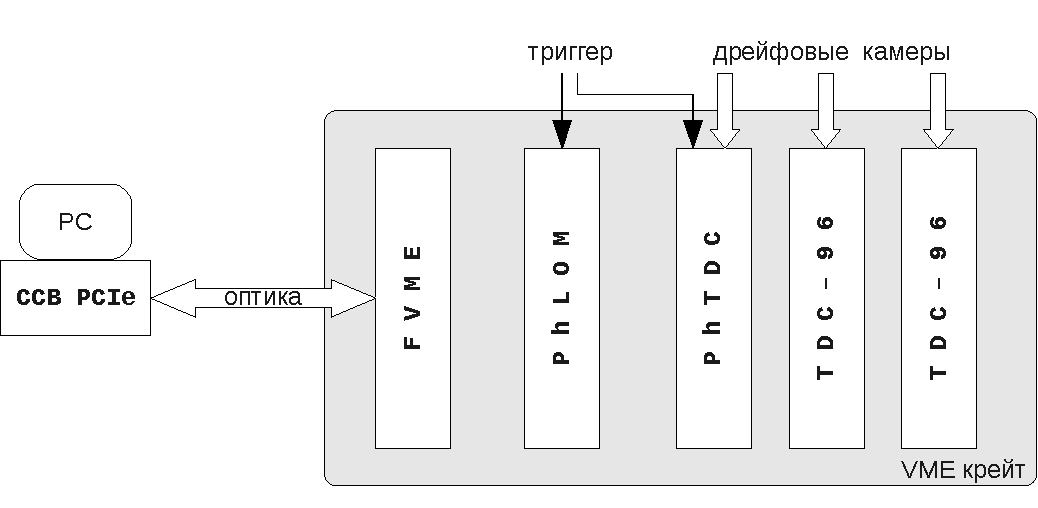
\includegraphics[width=0.95\textwidth]{modules_VME.pdf}
  \caption{Блок-схема системы сбора данных на установке. Сформированные сигналы
    с дрейфовых камер оцифровываются в модулях время-цифрового преобразования
    TDC-96 и PhTDC. Триггерный сигнал поступает на модули PhLOM и
    PhTDC. Интерфейсный FVME контроллер обеспечивает связь VME с удалённым
    компьютером по высокоскоростной оптической линии.}
  \label{fig:modules_VME.pdf}
\end{figure}

Система сбора данных в крейте VME включает в себя разные модули: интерфейсный,
триггерный и TDC. Интерфейсный модуль разработан для передачи данных и
возможности управления системой VME с удалённого компьютера. Контроллер крейта
(тип FVME) соединён по оптической линии с высокоскоростной M-Link сетевой
картой (тип CCB-PCIe) которая вставляется в PCI Express слот компьютера.
Оптическая линия передачи даёт возможность дуплексного обмена данными с большой
скоростью 200~МБ/с на расстоянии до 500 метров при использовании оптического
кабеля.

Триггерный модуль (тип PhLOM) имеет пять логических линий, один тестовый
сигнал, программируемую логику совпадений и счётчики импульсов на входе. Для
системы считывания данных используются выходные сигналы с программируемой
задержкой, которая определяется временем прохождения частицы через установку.
После прихода внешнего триггерного сигнала, в пределах запрограммированного
временного окна, проводится сбор данных по всем каналам.

TDC модули (время-цифровые преобразователи) применяются для преобразования \!
(оцифровки) времени сформированных \! импульсных сигналов с дрейфовых камер. На
данный момент используются три TDC модуля. Один 64-канальный модуль (тип PhTDC)
и два 96-канальные модуля (тип TDC-96). Данные модули разработаны на базе
специализированной интегральной схемы HPTDC~\cite{hptdc04}. Это 32-канальный чип
время-цифрового преобразования с разрешением до 25 пс и оцифровкой обоих фронтов
импульсов.

\section{Система запуска установки, триггер}
\label{section:trigger}
Система запуска установки или отбора событий (триггерная система) в процессе
измерений является необходимой составляющей эксперимента. Триггер установки
СТРЕЛА должен обеспечить набор событий реакции развала дейтрона при нулевом
(близком к нулю) угле рассеяния дейтрона на протоне. В нашем случае
регистрируются два протона с близкими импульсами и малым углом раствора из
реакции перезарядки дейтрона на протоне \dpchex (развал дейтрона с зарядовым
обменом) и однопротонные события из реакции прямого развала дейтрона \dpret.
Доля двухпротонных событий по отношению к однопротонным, при рассеянии на малые
углы, в нашем интервале энергий составляет приблизительно от 10$^{-4}$ до
10$^{-3}$. Однопротонные события~--- это протоны спектаторы и их регистрация
является дополнительным процессом для нормировки дифференциального сечения.

Запуск установки осуществлялся с помощью триггерных счётчиков~--- три
сцинтилляционных счётчика S1--S3 со сцинтилляторами на основе полистирола.
Размеры сцинтилляторов в счётчиках: S1~--- 10~$\times$ 10~$\times$ 0.5~см$^3$,
S2~--- 7~$\times$ 7~$\times$ 0.5~см$^3$ и S3~--- 25~$\times$ 22~$\times$
1.0~см$^3$. Световоды изготовлены из оргстекла. Для считывания света применялись
фотоумножители XP\,2020. Счётчик S3, имеющий сцинтиллятор большой площади,
просматривается двумя ФЭУ для улучшения светосбора и, соответственно, повышения
эффективности регистрации прохождения частиц. Конструкция данного счётчика
показана на рис.~\ref{fig:scintilator_S3}. Счётчики S1 и S2 с одним ФЭУ сделаны
аналогично.

\begin{figure}[h]
  \centering
  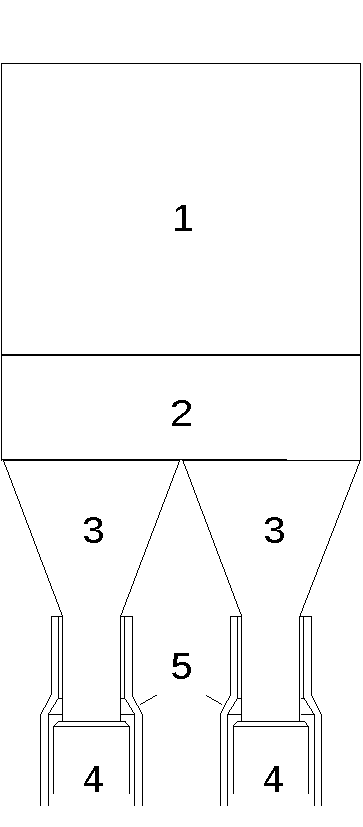
\includegraphics[width=0.32\textwidth]{scintilator_S3.pdf}
  \caption{Конструкция сцинтилляционного счётчика S3 с двумя фотоумножителями.
    1~--- сцинтиллятор (25~$\times$ 22~$\times$ 1.0~см$^3$), 2~и~3~--- световоды
    (оргстекло), 4~--- фотоумножители (XP2020), 5~--- магнитные экраны.}
  \label{fig:scintilator_S3}
\end{figure}

Сцинтилляционные счётчики S1--S3 определяют аксептанс установки и вырабатывают
сигнал для открытия временного окна регистрации сигналов с дрейфовых камер и
запуска системы сбора данных. Сигналы с фотоумножителей
поступают на входы формирователей со следящим порогом. Использование данных
формирователей позволяет скомпенсировать временной разброс сигналов, вызванный
передним фронтом амплитуды сигнала поступающего с ФЭУ. Временная и амплитудная
информация со счётчиков оцифровывается и записывается в каждом событии для
последующего контроля работоспособности счётчиков и всей триггерной системы.

Схема быстрой электронной логики системы запуска считывания данных, используемая
на установке, представлена на рис.~\ref{fig:trigger_scheme}. После
формирователей со следящим порогом логические сигналы поступают на схему
совпадений. В случае совпадения сигналов от всех триггерных счётчиков S1--S3,
вырабатывается сигнал запуска системы считывания данных и событие
регистрируется. Данный триггерный сигнал разветвляется и поступает на вход
триггерного модуля PhLOM VME крейта, на вход модуля TDC VME крейта и на схему
запрета, которая блокирует повторное срабатывание до окончания процесса сбора
данных в контроллер VME крейта. После появления триггерного сигнала проводится
сбор информации (раздел~\ref{section:electro}) по всем каналам дрейфовых камер.

\begin{figure}[h]
  \centering
  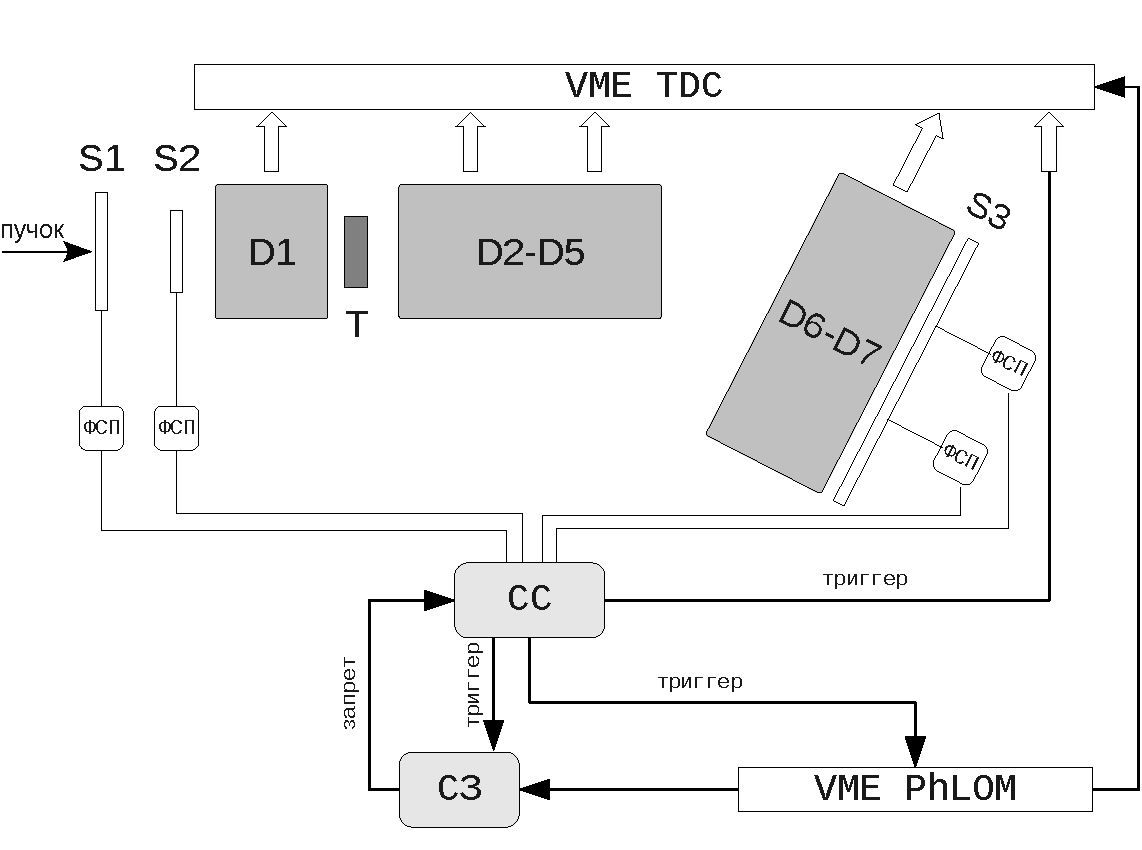
\includegraphics[width=1.00\textwidth]{trigger_scheme.pdf}
  \caption{Схема системы запуска (триггер) считывания данных на установке
    СТРЕЛА. S1--S3~--- сцинтилляционные счётчики, D1--D7~--- блоки дрейфовых
    камер (блоки D6--D7 расположенные после магнита), T~--- мишень, ФСП~---
    формирователь со следящим порогом, СС~--- схема совпадений, СЗ~--- схема
    запрета, VME~TDC~--- модуль время-цифрового преобразования, VME~PhLOM~---
    триггерный модуль.}
  \label{fig:trigger_scheme}
\end{figure}

Во время набора данных, наблюдалась устойчивая работа системы в течение всего
сеанса. Число принимаемых событий за один цикл сброса пучка из ускорителя на
мишень может достигать приблизительно 7500 событий. Среднее число слов, при
регистрации однопротонного события, равно 37 (регистрируемый протон проходит
все 36 плоскостей дрейфовых камер + триггерный сигнал).

Следует отметит, что используемый в данный момент триггер неидеален. Он
обеспечивает приём информации о всех событиях, в том числе и со стриппинговыми
протонами из реакции прямого развала дейтрона, доля которых достаточно велика.
Отбор двухтрековых событий из реакции перезарядки проводится только в процессе
offline обработки, что значительно увеличивает время анализа набранной
информации. Поэтому, желательно было бы организовать специальный триггер, для
отбора двухтрековых событий, используя информацию с дрейфовых камер, однако, это
требует разработки специализированных временных модулей.

\section{Анализирующий магнит}
В качестве анализирующего магнита используется дипольный электромагнит 2СП-40,
расположенный на канале ВП-1 после фокуса Ф5 (рис.~\ref{fig:channel_VP1}) с
поперечными размерами 100~$\times$~30~см$^2$. Магнит создаёт необходимое
магнитное поле в интервале 0.7--1.0~Т на протяжении 150 см, вдоль пути
прохождения частиц. Анализирующий магнит разводит в пространстве
непровзаимодействовавший пучок дейтронов и регистрируемые протоны из реакции
dp-взаимодействия, которые направляются на блоки больших дрейфовых камер.
Радиус кривизны траектории протонов стриппинга в магните равен приблизительно
7~м при значении магнитной индукции 0.83~Т.

\begin{figure}[h]
  \centering
  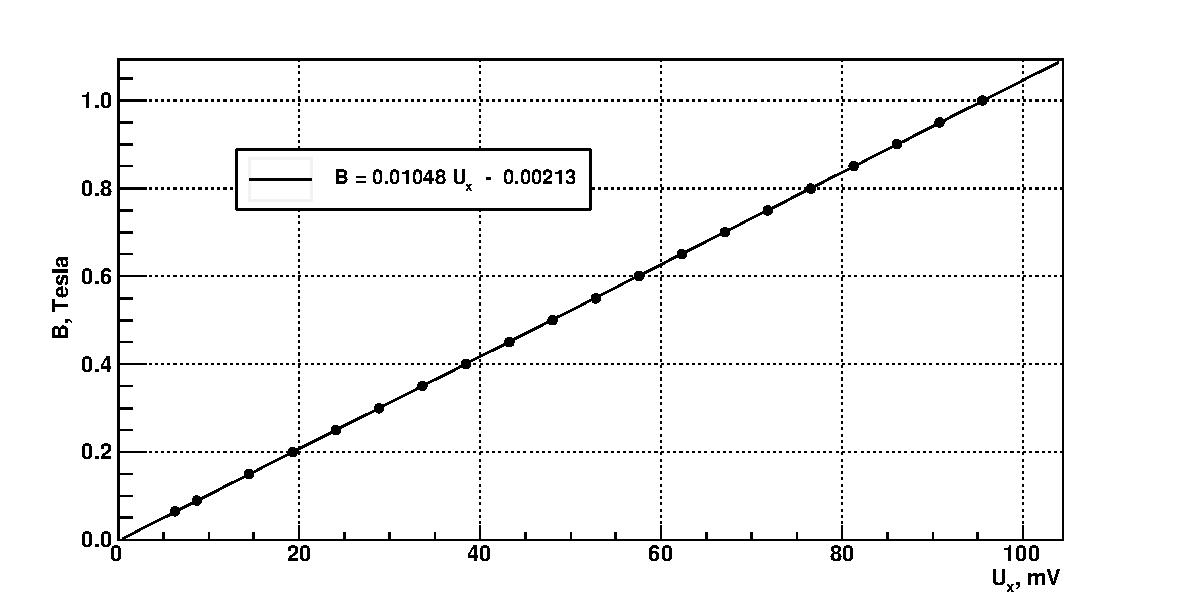
\includegraphics[width=1.00\textwidth]{magnet_hall_calib.pdf}
  \caption{Калибровка датчика Холла ДХ\,10.}
  \label{fig:magnet_hall_calib}
\end{figure}

Контроль и измерение магнитного поля в магните осуществляется датчиком Холла
(модель ДХ\,10), расположенным непосредственно на полюсе электромагнита. Датчик
перед началом измерений был прокалиброван, рис.~\ref{fig:magnet_hall_calib}.
Зависимость между сигналом датчика (холловским выводом) и магнитной индукцией
была строго линейна и аппроксимировалась выражением
\begin{equation}
  B = 0.01048\,U_{x} - 0.00213\,,
\end{equation}
где $B$~--- магнитная индукция в единицах Тесла и $U_{x}$~--- значение выходного
сигнала датчика Холла в мВ.

\begin{figure}[h]
  \centering
  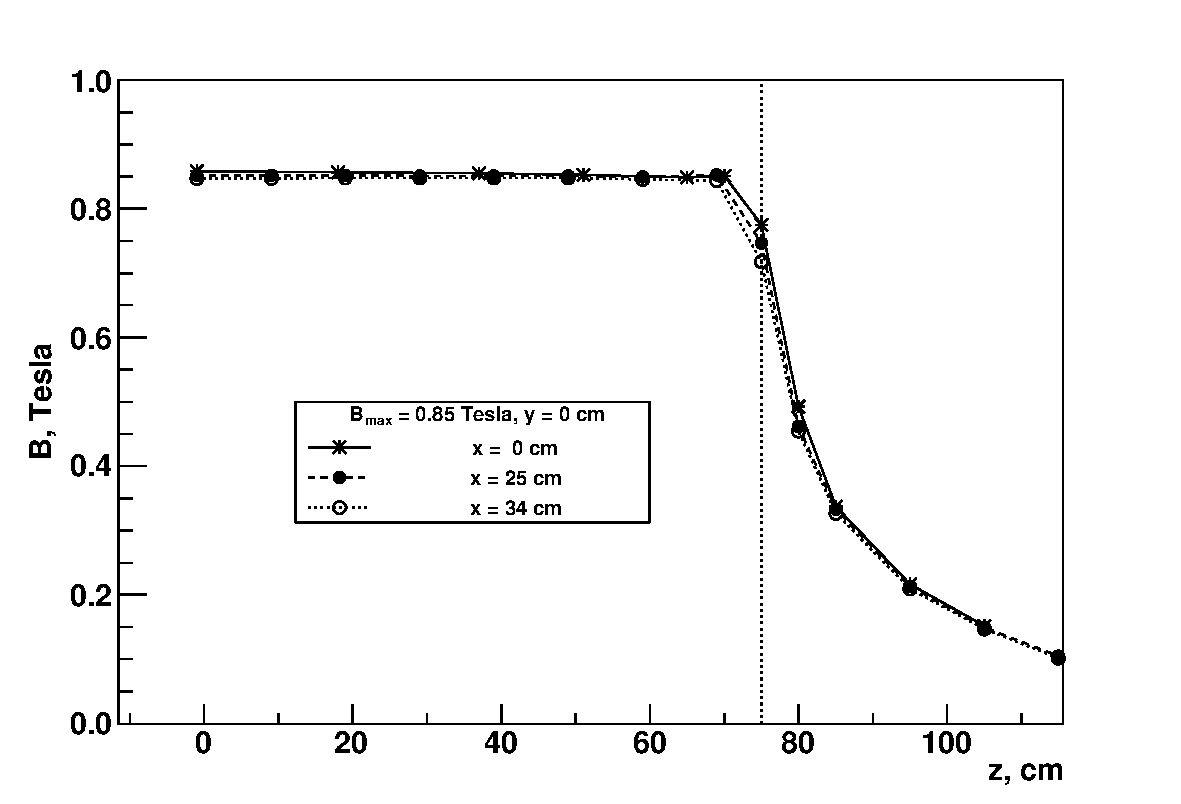
\includegraphics[width=1.00\textwidth]{magnet_eff.pdf}
  \caption{Зависимость магнитного поля $B$ магнита 2СП-40 от $z$-координаты
    для трёх разных значений $x$-координаты в медиальной плоскости $y=0$~см.
    Пунктирная линия означает координату конца полюса магнита ($z=75$~см).}
  \label{fig:magnet_eff}
\end{figure}

Измерения магнитного поля проводились между полюсами магнита 2СП-40 при значении
максимальной индукции в центре магнита 0.85~Т. В медиальной плоскости ($y=0$~см)
снималось по 14 точек вдоль оси $z$ для трёх разных значений $x$-координаты
0~см, 25~см и 34~см. Использовалась такая же координатная система как для
дрейфовых камер (ось $z$ направлена по пучку падающих дейтронов, и вместе с
осями $x$ и $y$ составляют правую тройку). Распределение магнитного поля $B$
вдоль оси $z$ показано на рис.~\ref{fig:magnet_eff}.

Проведённые магнитные измерения показали неоднородность магнитного поля на краях
полюса. Учёт краевых эффектов на полюсах компенсировался увеличением эффективной
длины $L_{eff}$ магнитной дорожки о
\begin{equation}
  \Delta\,L_{eff} = \frac{\int\limits_{L_{1}}^{L_{0}} B(z)\,dz}{B_{max}}\,,
\end{equation}
где $L_{1}$~--- конец области максимального магнитного поля (край полюса
магнита), $L_{0}$~--- конец действия поля и $B_{max}$~--- индукция в центре
магнита. В результате эффективная длина анализирующего магнита 2СП-40 была
увеличена на $\Delta\,L_{eff} = 17.5$~см с каждой стороны (на входе и выходе
частицы в магнит) и составила 185 см. В рабочей области магнита поле оказалось
достаточно однородным. Однако, стоит заметить, что в дальнейшем было бы
желательно провести более точное измерение магнитного поля и составить полную
трёхмерную карту распределения всех компонент вектора магнитного поля.

\section{Облучение аппаратуры СТРЕЛА}
Изучение характеристик всех блоков дрейфовых камер (кроме повёрнутых камер)
экспериментальной установки СТРЕЛА было проведено при облучении полиэтиленовой
мишени диаметром 5~см коллимированным пучком дейтронов с импульсом 3.5~ГэВ/с
на канале ВП-1 ускорительного комплекса Нуклотрона ЛФВЭ ОИЯИ. Сеанс работы
ускорителя состоялся в марте 2007 года. Аппаратура установки проверялась в
течение почти двух суток. Работа повёрнутых блоков дрейфовых камер D3 и D7
(рис.~\ref{fig:strela_setup}), которые были приобретены позже, была
дополнительно испытана с $\beta$-источником.

Система стабилизации интенсивности выведенного пучка из ускорителя обеспечивает
равномерную интенсивность не ниже $\sim 10^{7}$ частиц в секунду. Так как
дрейфовые камеры могут работать при интенсивности не больше $\sim 10^{6}$ частиц
в секунду, то для уменьшения интенсивности использовался стальной коллиматор с
отверстием прямоугольной формы размером 4~$\times$ 4~мм$^2$ и длиной 1.2~м,
устанавливаемый в районе фокуса Ф3 после поворотного магнита СП-94 канала ВП-1
(рис.~\ref{fig:channel_VP1}). Применение коллиматора позволило при интенсивности
пучка в фокусе Ф3 на уровне $\sim 10^{7}$ частиц в секунду обеспечить
интенсивность пучка дейтронов на мишени установки в районе фокуса Ф5 на
уровне $\sim 5 \times 10^{5}$ частиц в секунду.

\vspace{-0.1cm}
\begin{figure}[h]
  \centering
  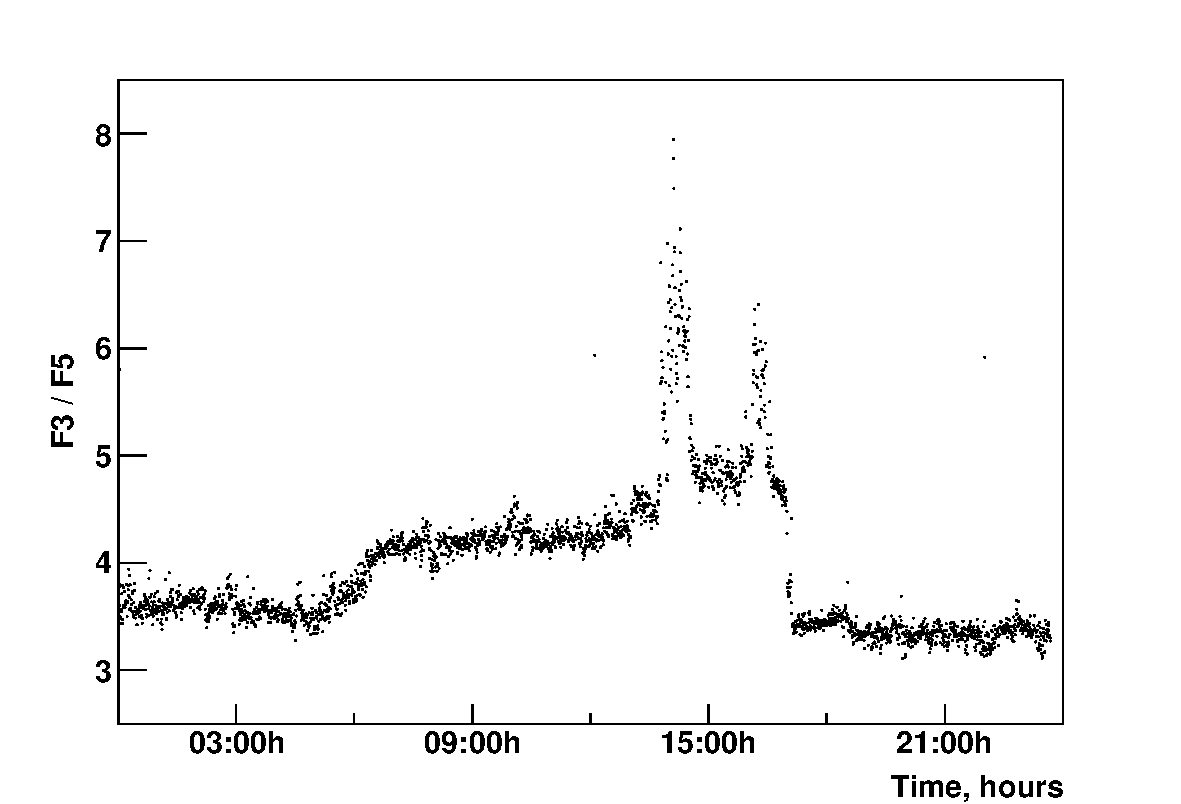
\includegraphics[width=1.00\textwidth]{beam_intensity.pdf}
  \caption{Изменение интенсивности выведенного дейтронного пучка на накале ВП-1
    в течение времени набора данных. Показано отношение счетов ионизационных
    камер, помещённых в фокусе Ф3 и Ф5 в зависимости от времени.}
  \label{fig:beam_intensity}
\end{figure}

Контроль интенсивности выведенного пучка осуществлялся с помощью ионизационных
камер. В процессе набора экспериментальных данных выявились нестабильности
выведенного пучка дейтронов. На рис.~\ref{fig:beam_intensity} приведено
отношение счетов с ионизационных камер расположенных в фокусах Ф3 и Ф5 в
зависимости от времени набора статистики. Повторные выбросы интенсивности пучка
приводили иногда к сбоям работы источников высоковольтного питания дрейфовых
камер. Использование коллиматора косвенно решает и задачу получения лучшей
временной структуры пучка.

В результате облучения аппаратуры установки СТРЕЛА было набрано несколько
миллионов триггеров для последующего анализа. Записанные события сначала
декодировались. Затем происходил поиск и реконструкция треков в дрейфовых
камерах. Более подробное описание процедуры обработки  полученных
экспериментальных данных будет приведено в следующей главе.

\section{Выводы к третьей главе}
Основные выводы данной главы можно сформулировать следующим образом:
\begin{list}{\labelitemi}{\leftmargin=1em}
\item Используя результаты исследований с помощью водородной
  пузырьковой камеры нами был предложен электронный эксперимент СТРЕЛА для
  изучения реакции перезарядки на дейтроне \dpchex с целью определения
  спин-зависящей части амплитуды элементарной перезарядки \np.
\item При активном участии диссертанта была создана экспериментальная установка
  СТРЕЛА и подробно описаны её основные компоненты.
\item Подробно освещены принципы работы и конструкции используемых дрейфовых
  камер, как наиболее важного элемента установки. Проведены испытания всех
  блоков дрейфовых камер и проверена их работа.
\item Обсуждены вопросы считывания информации, системы сбора данных с помощью
  быстрой электроники в формате стандарта VME и запуска установки.
\item Впервые проведено \! облучение установки в пучке релятивистских дейтронов
  импульса 3.5 ГэВ/с на ускорительном комплексе Нуклотрона ЛФВЭ ОИЯИ.
\end{list}

%%% Local Variables:
%%% mode: latex
%%% TeX-master: "musinsky_disser"
%%% coding: utf-8
%%% End:
